\documentclass[conference]{IEEEtran}
\IEEEoverridecommandlockouts
\usepackage{amsmath,amssymb,bm}
\usepackage{graphicx}
\usepackage{booktabs,array,multirow}
\usepackage[caption=false,font=footnotesize]{subfig}
\usepackage{microtype}
\usepackage{cite}
\usepackage{siunitx}
\usepackage{balance}
\usepackage{tikz}
\usetikzlibrary{arrows.meta,positioning,fit}
\sisetup{detect-all, per-mode=symbol}

\interdisplaylinepenalty=2500
\setcounter{dbltopnumber}{2}
\renewcommand{\dbltopfraction}{0.92}
\renewcommand{\textfraction}{0.05}
\renewcommand{\dblfloatpagefraction}{0.85}

\newcommand{\R}{\mathbb{R}}
\newcommand{\T}{^{\mathsf T}}
\newcommand{\I}{\mathbf I}
\newcommand{\diag}{\operatorname{diag}}
\newcommand{\norm}[1]{\left\lVert#1\right\rVert}

\begin{document}

\title{Nonlinear State Estimation and Constrained Trajectory Tracking of a Quadrotor Using EKF--NMPC}

\author{\IEEEauthorblockN{Gandham Lohith Varma, Gao Ningbo, Yang Jiaxin}
\IEEEauthorblockA{Group 8, MA6224\\
Nanyang Technological University, Singapore}}

\maketitle

\begin{abstract}
This paper presents a guidance, navigation, and control stack for a six-degree-of-freedom quadrotor tracking a three-dimensional lemniscate. A 13-state extended Kalman filter (EKF) propagates the nonlinear rigid-body model and sequentially fuses inertial and GNSS measurements. A constrained nonlinear model predictive controller (NMPC), formulated with direct multiple shooting, computes the four rotor-thrust commands from the EKF estimate alone. Two solver implementations are evaluated: a baseline CasADi/IPOPT formulation and a final acados formulation using SQP-RTI. In a 60-s MuJoCo simulation, the final acados-based closed loop achieves centimetre-level tracking, estimation errors that remain largely within their $\pm2\sigma$ envelopes, and rotor commands that stay within the prescribed limits. The acados solver requires \SI{0.95}{ms} on average and \SI{15.35}{ms} at maximum, satisfying the \SI{50}{ms} solver deadline in simulation.
\end{abstract}

\begin{IEEEkeywords}
Quadrotor, extended Kalman filter, nonlinear model predictive control, sensor fusion, constrained optimization.
\end{IEEEkeywords}

%==================================================================
\section{System Architecture and Mission}
%==================================================================
The closed loop comprises a MuJoCo plant~\cite{todorov2012mujoco}, simulated IMU and GNSS sensors, a 13-state EKF, and an NMPC trajectory-tracking controller (Fig.~\ref{fig:arch}). The controller receives only the corrected EKF estimate, never the simulated true state. Execution rates are listed in Table~\ref{tab:params}.

\begin{figure}[!b]
\centering
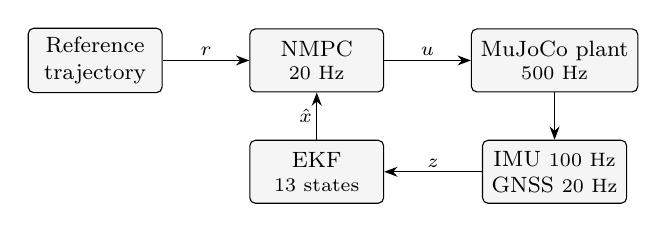
\begin{tikzpicture}[font=\footnotesize, >=Stealth, node distance=6mm and 11mm,
  blk/.style={draw, rounded corners=2pt, minimum height=8mm, minimum width=17mm, align=center, fill=gray!8},
  lab/.style={font=\scriptsize, align=center, inner sep=1.5pt}]
\node[blk] (ref) {Reference\\trajectory};
\node[blk, right=of ref] (mpc) {NMPC\\[-1pt]{\scriptsize 20 Hz}};
\node[blk, right=of mpc] (plant) {MuJoCo plant\\[-1pt]{\scriptsize 500 Hz}};
\node[blk, below=of plant] (sens) {IMU {\scriptsize 100 Hz}\\GNSS {\scriptsize 20 Hz}};
\node[blk, below=of mpc] (ekf) {EKF\\[-1pt]{\scriptsize 13 states}};
\draw[->] (ref) -- node[lab, above]{$r$} (mpc);
\draw[->] (mpc) -- node[lab, above]{$u$} (plant);
\draw[->] (plant) -- (sens);
\draw[->] (sens) -- node[lab, above]{$z$} (ekf);
\draw[->] (ekf) -- node[lab, left]{$\hat x$} (mpc);
\end{tikzpicture}
\caption{Closed-loop architecture: reference $r$, rotor-thrust command $u$, sensor measurements $z$, and EKF estimate $\hat x$. The controller uses only $\hat x$, and $u$ also drives the EKF prediction.}
\label{fig:arch}
\end{figure}

\textit{Frames.} The world frame is North--East--Down (NED) and the body frame is Forward--Right--Down (FRD). Gravity therefore acts along $+z_W$, every rotor produces thrust along $-z_B$, and $R_{WB}(q)$ maps body-frame vectors into the world frame. Quaternions are scalar-first, $q=[q_w,q_x,q_y,q_z]\T$.

\textit{Reference.} For $0\le t\le\SI{60}{s}$ the vehicle tracks
\begin{equation}
\begin{aligned}
x_r&=3\sin(0.25t), & y_r&=2\sin(0.5t),\\
z_r&=-2.5+0.5\cos(0.25t), & \psi_r&=\operatorname{atan2}(\dot y_r,\dot x_r),
\end{aligned}
\label{eq:reference}
\end{equation}
where the negative $z_r$ corresponds to an altitude of 2.0--3.0~m in NED.

\textit{Sensors.} The IMU contains white noise and random-walk biases; GNSS contains white position noise:
\begin{equation}\setlength{\arraycolsep}{0pt}\medmuskip=2mu\thickmuskip=3mu
\begin{aligned}
z_{a,k}&=f_{B,k}+b_{a,k}+n_{a,k}, & z_{G,k}&=p_{W,k}+n_{G,k},\\
z_{g,k}&=\omega_{B,k}+b_{g,k}+n_{g,k}, & b_{\ast,k+1}&=b_{\ast,k}+\sigma_{b\ast}\sqrt{\Delta t}\,\eta_{\ast,k}
\end{aligned}
\label{eq:sensors}
\end{equation}
where $\ast\in\{a,g\}$, $f_B=R_{WB}\T(a_W-g_W)$ is the specific force sensed by the accelerometer, and $\eta\sim\mathcal N(0,\I)$. All numerical values are collected in Table~\ref{tab:params}.

\begin{table}[t]
\caption{Model Parameters, Operating Limits, Sensor Noise, and Rates}
\label{tab:params}
\centering\footnotesize
\setlength{\tabcolsep}{3pt}
\begin{tabular}{@{}llc@{}}
\toprule
Quantity & Symbol & Value \\
\midrule
\multicolumn{3}{@{}l}{\textit{Vehicle}}\\
Mass & $m$ & \SI{1.20}{kg} \\
Arm lengths & $d_x,d_y$ & \SI{0.225}{m} \\
Roll/pitch inertia & $J_{xx},J_{yy}$ & \SI{1.25e-2}{kg.m^2} \\
Yaw inertia & $J_{zz}$ & \SI{2.20e-2}{kg.m^2} \\
Torque/thrust ratio & $c_\tau$ & \SI{0.015}{m} \\
\midrule
\multicolumn{3}{@{}l}{\textit{Operating limits}}\\
Rotor thrust & $T_i$ & $[0.2,\,5.5]$~N \\
Collective thrust & $T$ & $[0.8,\,22.0]$~N (hover \SI{11.77}{N}) \\
Roll/pitch angle & $\phi,\theta$ & $\pm35^\circ$ \\
Body rates & $p,q,r$ & $\pm180,\ \pm180,\ \pm90$~$^\circ$/s \\
\midrule
\multicolumn{3}{@{}l}{\textit{Sensor noise (standard deviation)}}\\
Accelerometer & $\sigma_a$ & \SI{0.08}{m/s^2} \\
Gyroscope & $\sigma_g$ & \SI{0.015}{rad/s} \\
GNSS position & $\sigma_G$ & \SI{0.02}{m} \\
Accel./gyro bias walk & $\sigma_{ba},\sigma_{bg}$ & $2\times10^{-3}$, $2\times10^{-4}$ \\
\midrule
\multicolumn{3}{@{}l}{\textit{Execution rates}}\\
MuJoCo integration & -- & \SI{500}{Hz} \\
EKF prediction, IMU correction & -- & \SI{100}{Hz} \\
GNSS correction, NMPC & -- & \SI{20}{Hz} \\
\bottomrule
\end{tabular}
\end{table}

%==================================================================
\section{Nonlinear Quadrotor Model}
%==================================================================
\subsection{State, Input, and Rotor Wrench}
The state and input are
\begin{equation}
\begin{aligned}
x&=\begin{bmatrix}p_W\T & v_W\T & q_{WB}\T & \omega_B\T\end{bmatrix}\T\in\R^{13},\\
u&=\begin{bmatrix}T_0 & T_1 & T_2 & T_3\end{bmatrix}\T\in\R^{4}.
\end{aligned}
\label{eq:stateinput}
\end{equation}
For the X configuration of Fig.~\ref{fig:rotormodes}, the collective force and body torques are
\begin{equation}
\begin{bmatrix}F_z\\ \tau_x\\ \tau_y\\ \tau_z\end{bmatrix}
=\begin{bmatrix}
-1 & -1 & -1 & -1\\
-d_y & -d_y & d_y & d_y\\
-d_x & d_x & d_x & -d_x\\
-c_\tau & c_\tau & -c_\tau & c_\tau
\end{bmatrix} u
\label{eq:mixer}
\end{equation}
with $T_B=[0,\,0,\,F_z]\T$. The first row is negative because thrust acts along $-z_B$. Equal rotor thrusts cancel all torques; $T_i=mg/4=\SI{2.943}{N}$ gives hover, and differential thrust produces roll, pitch, or yaw (Fig.~\ref{fig:rotormodes}).

\begin{figure}[t]
\centering
\includegraphics[width=\columnwidth]{figures/rotor_modes.png}
\caption{Rotor-thrust patterns for the implemented X configuration and $T_0$--$T_3$ numbering. Red, dark blue, and light blue denote high, hover, and low thrust.}
\label{fig:rotormodes}
\end{figure}

\subsection{Continuous-Time Dynamics}
The rigid-body model is
\begin{equation}
\begin{aligned}
\dot p_W &= v_W, &
\dot v_W &= \tfrac{1}{m}R_{WB}(q)\,T_B+g_W,\\
\dot q_{WB} &= \tfrac12\,q_{WB}\otimes[0,\;\omega_B\T]\T, &
\dot\omega_B &= J^{-1}(\tau_B-\omega_B\times J\omega_B).
\end{aligned}
\label{eq:continuous}
\end{equation}
with $\tau_B=[\tau_x,\tau_y,\tau_z]\T$. Collective thrust, rotated into the world frame, drives translation; differential thrust drives angular acceleration, which in turn drives attitude through the quaternion kinematics. The EKF and the baseline CasADi/IPOPT NMPC discretize~\eqref{eq:continuous} with fourth-order Runge--Kutta (RK4) followed by quaternion normalization. The final acados NMPC instead uses a four-stage explicit Runge--Kutta integrator inside the generated solver. The resulting discrete transition is denoted $f_d(x,u)$.

%==================================================================
\section{Extended Kalman Filter}
%==================================================================
\subsection{Estimation Cycle}
Each cycle predicts with the model and then corrects sequentially with the IMU and, when available, GNSS:
\begin{equation}
\begin{aligned}
(\hat x_k,P_k)&\xrightarrow{\text{predict}}(\hat x^-_{k+1},P^-_{k+1})\\
&\xrightarrow{\text{IMU}}(\hat x^I_{k+1},P^I_{k+1})
\xrightarrow{\text{GNSS}}(\hat x_{k+1},P_{k+1}).
\end{aligned}
\label{eq:ekfflow}
\end{equation}
The quaternion is normalized after every step.

\subsection{Prediction}
The state and covariance are propagated as
\begin{equation}
\hat x^-_{k+1}=f_d(\hat x_k,u_k),\qquad
P^-_{k+1}=F_kP_kF_k\T+Q,
\label{eq:predict}
\end{equation}
where $F_k=\partial f_d/\partial x\,|_{\hat x_k}$ is the Jacobian of the full RK4 step, evaluated by central differences. Because $F_k$ is taken from the same discrete map that propagates the state, the covariance and state propagation are consistent. The first term of~\eqref{eq:predict} redistributes existing uncertainty through the dynamics; $Q$ is the only source of new uncertainty per step. Since $Q$ is applied without a $\Delta t$ factor, it is a per-step (discrete) covariance.

The initial and process covariances are
\begin{align}
P_0&=\diag\!\left(0.2^2\I_3,\;0.2^2\I_3,\;0.05^2\I_4,\;0.1^2\I_3\right),\label{eq:P0}\\
Q&=\diag\!\left(10^{-6}\I_3,\;10^{-4}\I_3,\;10^{-7}\I_4,\right.\nonumber\\
&\qquad\left.10^{-4},\;10^{-4},\;3\!\times\!10^{-5}\right).\label{eq:Q}
\end{align}
$P_0$ assigns initial standard deviations of \SI{0.2}{m}, \SI{0.2}{m/s}, 0.05 per quaternion component, and \SI{0.1}{rad/s}. The small position and quaternion entries of $Q$ reflect their purely kinematic propagation; the larger velocity and rate entries absorb unmodelled forces and torques. Both matrices were tuned in simulation until the $\pm2\sigma$ envelopes were consistent with the observed errors without making the estimate noisy.

\subsection{Measurement Correction}
Both sensors use the same correction with their own model $h(\cdot)$, Jacobian $H=\partial h/\partial x$, and noise covariance $R$:
\begin{equation}
\begin{aligned}
\nu &= z-h(\hat x^{\ominus}), & S &= HP^{\ominus}H\T+R,\\
K &= P^{\ominus}H\T S^{-1}, & \hat x^{\oplus}&=\hat x^{\ominus}+K\nu,\\
A &= \I-KH, & P^{\oplus}&=AP^{\ominus}A\T+KRK\T,
\end{aligned}
\label{eq:update}
\end{equation}
where $\ominus$ and $\oplus$ denote the prior and posterior of that correction. The Joseph form preserves symmetry and positive semi-definiteness of $P$ even when $K$ is not exactly optimal.

\textit{IMU.} The predicted IMU output stacks specific force and body rate,
\begin{equation}
h_I(x,u)=\begin{bmatrix}R_{WB}\T(q)\bigl(\dot v_W(x,u)-g_W\bigr)\\ \omega_B\end{bmatrix},
\label{eq:hI}
\end{equation}
so the accelerometer term uses the full model rather than a quasi-static gravity-only approximation. $H_I$ is computed numerically at $\hat x^-_{k+1}$ and $R_I=\diag(0.08^2\I_3,\,0.015^2\I_3)$.

\textit{GNSS.} GNSS observes position directly, $h_G(x)=p_W$, so $H_G=[\I_3\;\;0_{3\times10}]$ and $R_G=0.02^2\I_3$. It is applied to the IMU-corrected pair $(\hat x^I_{k+1},P^I_{k+1})$. Although only position is measured, the cross-covariances in $P^I$ let the GNSS residual correct correlated velocity, attitude, and rate errors.

The IMU biases in~\eqref{eq:sensors} are present in the simulated measurements but are not included in the EKF state; this modelling mismatch is discussed in Section~\ref{sec:discussion}-B.

%==================================================================
\section{Nonlinear Model Predictive Controller}
%==================================================================
\subsection{Nonlinear Model Predictive Controller}
The NMPC is implemented using two numerical solution frameworks: a baseline CasADi/Ipopt nonlinear-programming implementation and an acados implementation using SQP-RTI. To permit a direct comparison of solver performance, both implementations retain the same nonlinear quadrotor model, state and control definitions, prediction horizon, tracking objective, cost weights, actuator limits, and flight-envelope constraints. Hence, the controller design is kept fixed while the numerical solution strategy is changed.

\subsection{Cost Function Design}
% At every \SI{50}{ms} control instant the NMPC predicts $N=20$ intervals ($T_p=\SI{1}{s}$). Predicted states and inputs are both decision variables (direct multiple shooting):
% \begin{equation}
% X_k=[x_{0|k},\dots,x_{N|k}],\qquad U_k=[u_{0|k},\dots,u_{N-1|k}].
% \label{eq:decision}
% \end{equation}
% With the tracking errors
% \begin{equation}
% \begin{aligned}
% e_{p,j}&=p_{j|k}-p_{r,j},\qquad e_{v,j}=v_{j|k}-v_{r,j},\\
% e_{\psi,j}^{sc}&=
% \begin{bmatrix}
% \sin\psi_{j|k}-\sin\psi_{r,j}\\
% \cos\psi_{j|k}-\cos\psi_{r,j}
% \end{bmatrix},
% \end{aligned}
% \label{eq:errors}
% \end{equation}
% where the sine--cosine embedding avoids the $\pm\pi$ discontinuity, and $u_h=(mg/4)\mathbf 1_4$ is the hover input.
% \begin{equation}
% \begin{aligned}
% \min_{X_k,U_k}\quad & \sum_{j=1}^{N-1}\ell_x(x_{j|k})+\sum_{j=0}^{N-1}\ell_u(u_{j|k})+\ell_N(x_{N|k})\\
% \text{s.t.}\quad & x_{0|k}=\hat x_k,\\
% & x_{j+1|k}=f_d(x_{j|k},u_{j|k}),\qquad j=0,\dots,N-1,\\
% & T_{\min}\le u_{j|k}\le T_{\max},\\
% & |\phi_{j|k}|,|\theta_{j|k}|\le35^\circ,\quad |\omega_{j|k}|\le\omega_{\max},
% \end{aligned}
% \label{eq:nlp}
% \end{equation}
% with stage, input, and terminal costs
% \begin{equation}
% \begin{aligned}
% \ell_x&=e_p\T Q_pe_p+e_v\T Q_ve_v+
% (e_\psi^{sc})\T Q_\psi e_\psi^{sc}
% +\omega\T Q_\omega\omega,\\
% \ell_u&=(u-u_h)\T R_u(u-u_h),\\
% \ell_N&=50\norm{e_{p,N}}_2^2+10\norm{e_{v,N}}_2^2
% +(e_{\psi,N}^{sc})\T Q_\psi e_{\psi,N}^{sc}
% +0.1\norm{\omega_N}_2^2.
% \end{aligned}
% \label{eq:cost}
% \end{equation}
% The state cost starts at $j=1$ because $x_{0|k}$ is fixed by the EKF estimate and cannot be influenced by the optimizer. Roll and pitch are obtained from the predicted quaternion, and the body-torque limits follow implicitly from the rotor-thrust bounds.
At each control instant, the predicted position, velocity, yaw, body rates, and rotor thrusts are penalized relative to their desired values. The position and velocity tracking errors are
\begin{equation}
e_{p,j}=p_{j|k}-p_{r,j},\qquad
e_{v,j}=v_{j|k}-v_{r,j},
\end{equation}
while the yaw error is wrapped to $[-\pi,\pi]$ as
\begin{equation}
e_{\psi,j}
=
\operatorname{atan2}
\left[
\sin(\psi_{j|k}-\psi_{r,j}),
\cos(\psi_{j|k}-\psi_{r,j})
\right].
\label{eq:yawerror}
\end{equation}
This avoids the artificial discontinuity that would otherwise occur
when the yaw angle crosses $\pm\pi$.

The nominal rotor input is the hover thrust
\begin{equation}
u_h=\frac{mg}{4}\mathbf{1}_4,
\end{equation}
which gives $T_i=\SI{2.943}{N}$ for the present vehicle.

For the predicted stages, the cost is
\begin{equation}
\begin{aligned}
\ell_j={}&
e_{p,j}^{\T}Q_pe_{p,j}
+
e_{v,j}^{\T}Q_ve_{v,j}
+
q_\psi e_{\psi,j}^{2}\\
&+
\omega_{j|k}^{\T}Q_\omega\omega_{j|k}
+
(u_{j|k}-u_h)^{\T}R_u(u_{j|k}-u_h),
\end{aligned}
\label{eq:stagecost}
\end{equation}

with
\begin{equation}
\begin{aligned}
Q_p&=\diag(30,30,40),\\
Q_v&=\diag(5,5,8),\\
q_\psi&=5,\\
Q_\omega&=0.1I_3,\\
R_u&=0.05I_4.
\end{aligned}
\label{eq:nmpcweights}
\end{equation}

The position terms receive the largest weights because path tracking is the primary control objective. The larger vertical position and velocity weights ($40$ and $8$) strengthen altitude regulation. Velocity penalties reduce overshoot, whereas the comparatively small body-rate penalty suppresses unnecessarily aggressive rotational motion without preventing attitude manoeuvres. Finally, $R_u$ regularizes the rotor commands about hover and discourages excessive differential thrust. The stronger terminal position and velocity penalties discourage the optimizer from postponing tracking error beyond the end of the prediction horizon.

The terminal penalty is
\begin{equation}
\ell_N
=
50\|e_{p,N}\|_2^2
+
10\|e_{v,N}\|_2^2.
\label{eq:terminalcost}
\end{equation}

\subsection{Controller Parameters and Solver Implementation}
Both implementations operate at a nominal NMPC period of
$\Delta t=\SI{0.05}{s}$ and use $N=20$ prediction intervals, giving a prediction horizon of
\begin{equation}
T_p=N\Delta t=\SI{1.0}{s}.
\end{equation}
At each solution, the current predicted state is fixed to the corrected EKF estimate,
\begin{equation}
x_{0|k}=\hat{x}_k,
\end{equation}
and subsequent states satisfy the nonlinear quadrotor dynamics.

Each rotor thrust is constrained by
\begin{equation}
\SI{0.2}{N}\le T_i\le\SI{5.5}{N},
\end{equation}
while the predicted flight envelope is limited to
\begin{equation}
|\phi|,|\theta|\le35^\circ,
\end{equation}
and
\begin{equation}
|p|,|q|\le180^\circ/\mathrm{s},
\qquad
|r|\le90^\circ/\mathrm{s}.
\end{equation}

The baseline implementation constructs the finite-horizon nonlinear program using CasADi and solves it with Ipopt. The nonlinear dynamics are discretized explicitly using fourth-order Runge--Kutta integration. The preceding optimal state and control trajectories are reused as initial guesses for the following solve.

For the real-time implementation, the same optimal-control objective and constraints are formulated in acados. The nonlinear program is solved using sequential quadratic programming with real-time iteration . Each resulting quadratic program is solved using HPIPM with partial condensing. Because the cost is implemented directly as an external nonlinear expression, the acados implementation uses the exact cost Hessian rather than the Gauss--Newton approximation used in the earlier nonlinear least-squares formulation.

The acados costs are implemented using the external cost type rather than reformulating the controller as nonlinear least squares. This permits the original wrapped-yaw stage cost and position--velocity terminal cost of the CasADi implementation to be reproduced directly.

\subsection{Solution}

CasADi~\cite{andersson2019casadi} is used to construct the baseline nonlinear program symbolically and provide the required derivatives, while IPOPT~\cite{wachter2006ipopt} solves the resulting optimization problem with at most 100 iterations and a tolerance of $10^{-4}$. The first solution is initialized around hover, and subsequent problems are warm-started using the preceding optimal state and input trajectories. Although this implementation provides satisfactory tracking performance, its computation time can exceed the \SI{50}{ms} control period.

For real-time execution, the same NMPC formulation is implemented in acados~\cite{verschueren2022acados}. The state and input definitions, prediction horizon, cost function, weighting matrices, terminal penalty, and physical constraints are retained so that the comparison mainly reflects the numerical solution method. The acados implementation uses SQP-RTI with an exact Hessian, partial condensing, and the HPIPM quadratic-program solver. The continuous-time model is integrated using a four-stage explicit Runge-Kutta scheme within the generated solver. To improve convergence, the previous optimal state and input trajectories are shifted forward by one prediction step and used to warm-start the next optimization.

Both implementations follow the receding-horizon principle and apply only the first element of the optimal input sequence,
\begin{equation}
u_k=u_{0|k}^{\star}.
\end{equation}
If a new optimization does not return a valid solution during real-time execution, the most recent valid rotor-thrust command is retained until a new feasible solution becomes available.

%==================================================================
\section{Simulation Results and Discussion}
\label{sec:discussion}
%==================================================================
No single plot can establish both observer and controller performance, so complementary metrics are used: trajectory overlap and tracking error for control accuracy, EKF error against its $\pm2\sigma$ envelope for estimator consistency, and rotor-thrust and body-torque histories to verify that accurate tracking is not obtained by violating actuator limits. The results are summarized in Table~\ref{tab:results} and Figs.~\ref{fig:tracking}--\ref{fig:ekf}.

\begin{figure*}[!p]
\centering
\subfloat[Three-dimensional trajectory]{
\includegraphics[width=0.485\textwidth,height=2.4in,keepaspectratio]{figures/3d_traj.png}\label{fig:traj}}\hfil
\subfloat[State-tracking errors]{
\includegraphics[width=0.485\textwidth,height=2.4in,keepaspectratio]{figures/state_tracking_error.png}\label{fig:trackerr}}\\[2pt]
\subfloat[Rotor-thrust commands]{
\includegraphics[width=0.485\textwidth,height=1.85in,keepaspectratio]{figures/rotor_thrust.png}\label{fig:thrust}}\hfil
\subfloat[Body-torque commands]{
\includegraphics[width=0.485\textwidth,height=1.85in,keepaspectratio]{figures/body_torque_commands.png}\label{fig:torque}}
\caption{Closed-loop tracking and actuation. (a)~Reference (blue) and flown (orange) paths. (b)~Position, velocity, and yaw tracking errors. (c)~Rotor thrusts with the $[0.2,5.5]$~N bounds. (d)~Body torques with the envelopes implied by the rotor-thrust bounds.}
\label{fig:tracking}
\end{figure*}

\begin{figure*}[!p]
\centering

\includegraphics[width=0.63\textwidth]{figures/ekf_estimation_error.png}
\caption{EKF estimation error (blue) with $\pm2\sigma$ envelopes from the diagonal of $P$ (dashed) for position, velocity, and body rates.}
\label{fig:ekf}
\end{figure*}

\begin{table}[t]
\caption{Principal Simulation Results (60-s run, Casadi)}
\label{tab:results}
\centering\footnotesize
\setlength{\tabcolsep}{4pt}
\begin{tabular}{@{}lc@{}}
\toprule
Metric & Result \\
\midrule
\multicolumn{2}{@{}l}{\textit{Tracking}}\\
Position RMSE $(x,y,z)$ & $(0.0137,\,0.0135,\,0.0089)$~m \\
\midrule
\multicolumn{2}{@{}l}{\textit{Estimation}}\\
EKF position RMSE $(x,y,z)$ & $(0.0104,\,0.0108,\,0.0107)$~m \\
$\pm2\sigma$ coverage $(p,q,r)$ & $(98.52,\,98.31,\,97.55)\%$ \\
\midrule
\multicolumn{2}{@{}l}{\textit{Actuation and flight envelope}}\\
Rotor-thrust range & $[1.542,\,4.574]$~N \quad (limit $[0.2,\,5.5]$) \\
Max.\ roll / pitch & $9.95^\circ$ / $6.37^\circ$ \quad (limit $35^\circ$) \\
Max.\ $|p|,|q|,|r|$ & $114.4,\;92.8,\;53.1$~$^\circ$/s \\
\midrule
\multicolumn{2}{@{}l}{\textit{Solver}}\\
NLP success rate & 100\% \\
Solving time, mean / max & $\approx0.09$~s / $\approx0.87$~s \\
\bottomrule
\end{tabular}
\end{table}

\begin{table}[t]
\caption{Principal Simulation Results (60-s run, Acados)}
\label{tab:results}
\centering\footnotesize
\setlength{\tabcolsep}{4pt}
\begin{tabular}{@{}lc@{}}
\toprule
Metric & Result \\
\midrule
\multicolumn{2}{@{}l}{\textit{Tracking}}\\
Position RMSE $(x,y,z)$ & $(0.0136,\,0.0134,\,0.0089)$~m \\
\midrule
\multicolumn{2}{@{}l}{\textit{Estimation}}\\
EKF position RMSE $(x,y,z)$ & $(0.0104,\,0.0108,\,0.0107)$~m \\
$\pm2\sigma$ coverage $(p,q,r)$ & $(98.47,\,98.45,\,97.62)\%$ \\
\midrule
\multicolumn{2}{@{}l}{\textit{Actuation and flight envelope}}\\
Rotor-thrust range & $[1.617,\,4.627]$~N \quad (limit $[0.2,\,5.5]$) \\
Max.\ roll / pitch & $10.14^\circ$ / $6.48^\circ$ \quad (limit $35^\circ$) \\
Max.\ $|p|,|q|,|r|$ & $116.6,\;94.7,\;54.5$~$^\circ$/s \\
\midrule
\multicolumn{2}{@{}l}{\textit{Solver}}\\
NLP success rate & 100\% \\
Solving time, mean / max & $\approx0.001$~s / $\approx0.015$~s \\
\bottomrule
\end{tabular}
\end{table}

\subsection{Performance}
\textit{Tracking.} The final casadi-based flown path overlaps the reference throughout (Fig.~\ref{fig:traj}), and the position RMSE remains at the centimetre level on every axis (Fig.~\ref{fig:trackerr}). The vertical error is the smallest, consistent with the larger $z$ weights. The yaw error is not zero-mean and reaches approximately $7^\circ$, indicating a persistent heading lag that follows the reference curvature.

\textit{Estimation.} The EKF position RMSE remains close to \SI{0.011}{m} on each axis. The estimation errors are approximately zero-mean and remain largely inside their $\pm2\sigma$ envelopes after the initial transient (Fig.~\ref{fig:ekf}), indicating that the estimator remains consistent under the final acados-based closed loop.

\textit{Constraints.} The rotor thrusts remain well inside $[0.2,5.5]$~N, apart from a brief transient at start-up (Fig.~\ref{fig:thrust}), and the body torques keep wide margins to their envelopes (Fig.~\ref{fig:torque}). The maximum roll and pitch angles are far below $35^\circ$, and all body rates stay within their limits.

\subsection{Limitations}
\textit{Real-time feasibility.} The baseline CasADi/IPOPT implementation required an average solution time of \SI{90.1}{ms} and a maximum of \SI{866}{ms}, exceeding the \SI{50}{ms} control period. To address this limitation, the NMPC was reimplemented in acados using SQP-RTI, partial condensing with HPIPM, generated solver code, and one-step-shifted warm starts. The resulting average and maximum solution times were reduced to \SI{0.95}{ms} and \SI{15.35}{ms}, respectively, while maintaining nearly identical tracking accuracy. The acados implementation therefore resolves the solver-side deadline violation in the present desktop simulation. However, only the NMPC solution time has been evaluated; complete end-to-end timing, including estimation, sensing, communication, operating-system scheduling, and actuator delays, remains to be validated on the target onboard hardware.

\textit{Unestimated IMU biases.} The simulated accelerometer and gyroscope biases follow random walks but are absent from the EKF state. Their effect is absorbed by $Q$ and, for position, corrected by GNSS. The bias magnitudes remain small over the 60-s run, but longer missions or GNSS outages would call for augmenting the state with $b_a$ and $b_g$ so that they are estimated explicitly.

%==================================================================
\section{Conclusion}
A 13-state EKF and a constrained NMPC were combined into a closed loop that tracks a three-dimensional lemniscate using estimated states only. The EKF fuses IMU and GNSS measurements through model-driven prediction, while the NMPC enforces rotor-thrust, attitude, and body-rate constraints. The baseline CasADi/IPOPT implementation achieved satisfactory tracking but failed to meet the \SI{50}{ms} solver deadline. Reimplementing the controller with acados SQP-RTI preserved centimetre-level tracking and constraint satisfaction while reducing the average and maximum solution times to \SI{0.95}{ms} and \SI{15.35}{ms}. The solver-side real-time requirement is therefore satisfied in simulation, while end-to-end validation on onboard hardware and bias-augmented state estimation remain future work.

\balance
\begin{thebibliography}{4}
\bibitem{todorov2012mujoco}
E.~Todorov, T.~Erez, and Y.~Tassa, ``MuJoCo: A physics engine for model-based control,'' in \emph{Proc. IEEE/RSJ Int. Conf. Intell. Robots Syst. (IROS)}, 2012, pp.~5026--5033.

\bibitem{andersson2019casadi}
J.~A.~E. Andersson, J.~Gillis, G.~Horn, J.~B. Rawlings, and M.~Diehl, ``CasADi: A software framework for nonlinear optimization and optimal control,'' \emph{Math. Program. Comput.}, vol.~11, no.~1, pp.~1--36, 2019.

\bibitem{wachter2006ipopt}
A.~W\"achter and L.~T. Biegler, ``On the implementation of an interior-point filter line-search algorithm for large-scale nonlinear programming,'' \emph{Math. Program.}, vol.~106, no.~1, pp.~25--57, 2006.

\bibitem{verschueren2022acados}
R.~Verschueren \emph{et al.}, ``acados---A modular open-source framework for fast embedded optimal control,'' \emph{Math. Program. Comput.}, vol.~14, pp.~147--183, 2022.
\end{thebibliography}

\end{document}
